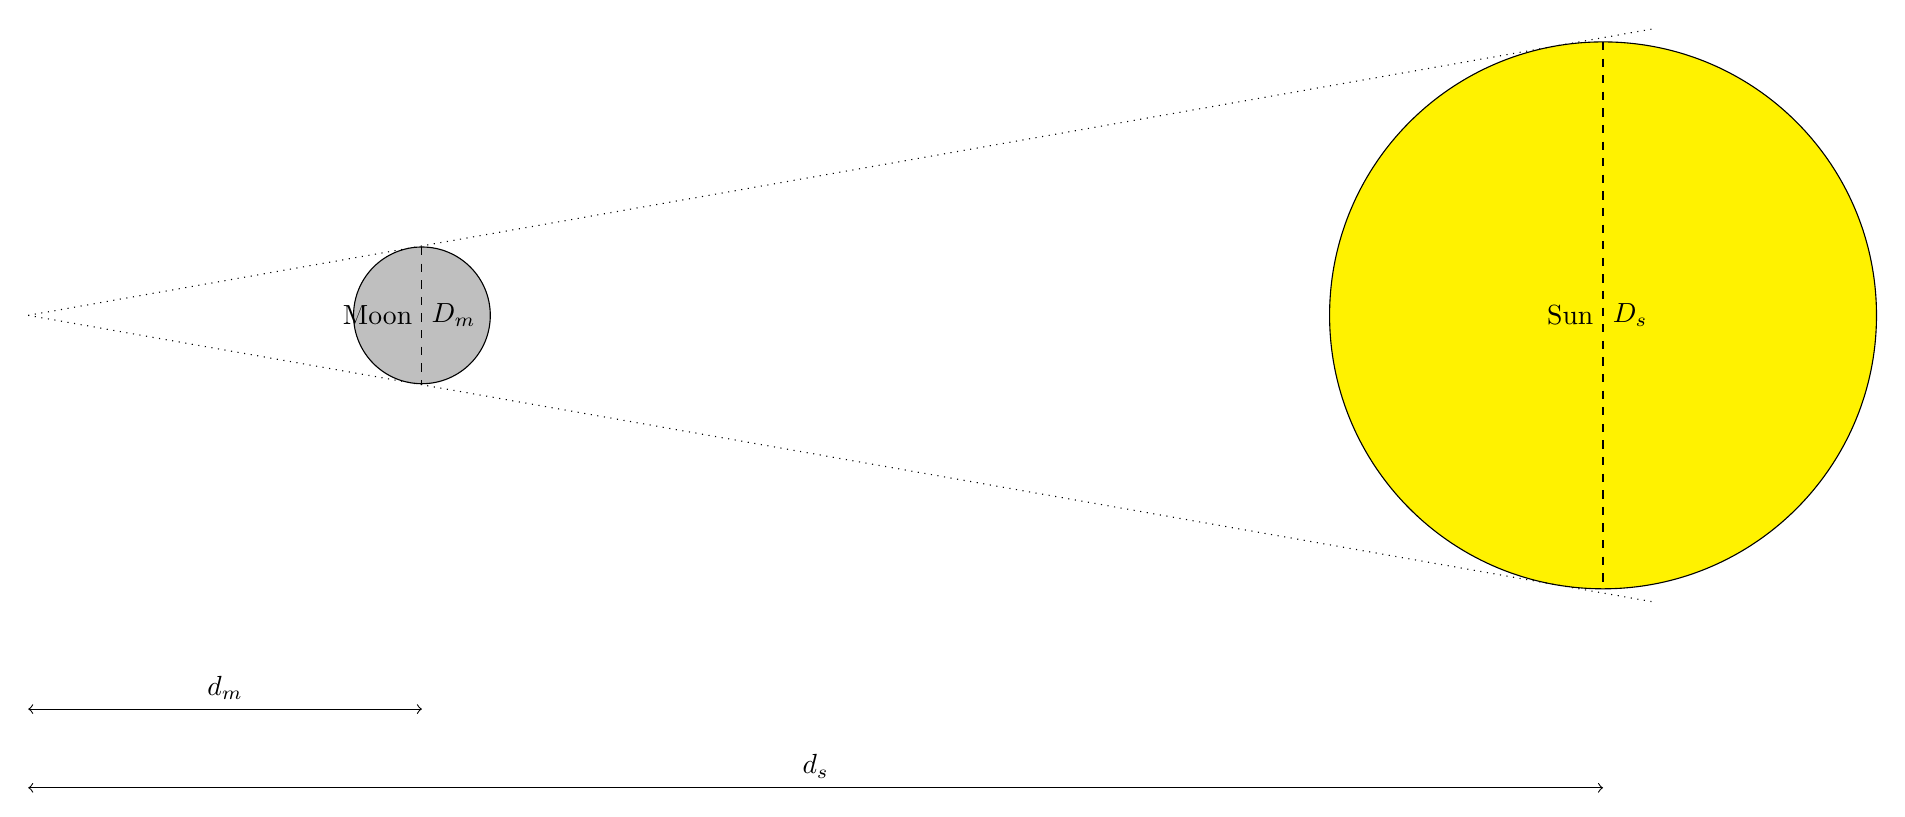
\begin{tikzpicture}[scale=1.0]

\def\eclipseangle{20}

% Sun 
\pgfmathparse{20*sin(10)}
\let\sunradius\pgfmathresult
\filldraw[fill=yellow] (20,0) circle (\sunradius) node[left] {Sun};
\draw[black,dashed] (20,\sunradius) -- (20,-\sunradius) node[midway,right] {$D_s$};

% Moon
\pgfmathparse{5*sin(10)}
\let\moonradius\pgfmathresult
\filldraw[fill=gray!50] (5,0) circle (\moonradius) node[left] {Moon};
\draw[black,dashed] (5,\moonradius) -- (5,-\moonradius) node[midway,right] {$D_m$};

% angle
%\draw[dotted] (20,\sunradius) -- (0,0) node {E} -- (20,-\sunradius);
\draw[dotted] (0,0) -- (10:21) (0,0) -- (-10:21);

% distances
\draw[<->] (0,-5) -- (5,-5) node[midway, above] {$d_m$};
\draw[<->] (0,-6)--(20,-6) node[midway, above] {$d_s$};

\end{tikzpicture}